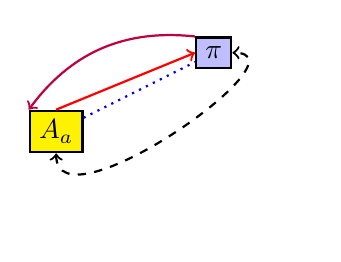
\begin{tikzpicture}
	%% Draw our two nodes -- note our content is mathematical
	\node at (0,0) [draw, thick, fill=yellow] (a) {$A_a$};		% Called `a'
	\node at (2,1) [draw, thick, fill=blue!25!white] (pi) {$\pi$};	% Called `pi'

	%% Connect up the node edges in various ways
	\draw [thick, dotted, blue] (a) -- (pi);	% Closest points
	\draw [thick, ->, red] (a.north) to (pi.west);	% `->' is an arrow
	\draw [thick, <->, dashed, out=-90, in=0] (a.south) to (pi.east); % Alternative bend mechanism
	\draw [thick, purple, bend left, <-] (a.north west) to (pi.north west);	% Yet another!
\end{tikzpicture}
